\chapter{Introduction}

%This chapter must contain presentation of 

%\begin{itemize}
%	\item context
%	\item problematic
%	\item company  activities
%	\item internship context 
%\end{itemize}

%The following organization can be used.



\section{Context}
Noise pollution is the disturb or loud noise may effected the activity or health of peole or
animal in life. Most of outdoor noise is mainly caused by machines and transportation
systems, motorbike engines, airplanes, and trains. Outdoor noise meaning is the
environmental noise: Urban planning or industrial areas are representation examples
Nowdays, noise levels can be main cause by cardiovascular illness or coronary artery in
human. For animals, noise can increase the count of death ,bad effected to reproduction
and hearing loss

\

Moreover, noise also appears in the images. Image noise is created by the sensor and
circuitry from scanner or digital camera. Film grain and noise of an ideal photon detector
are one of cause. So brightness or color information in images will be changed. Image
noise is unlike by product of image capture that have many different information.

\

Next, it is quality of camera. Although camera technology is very improve over the past
decade, it still has not totally remove noise for images. So now, researchers still find to
way which improve about camera to help us have image is better. Noise can appear in our
photo for different reasons. Noise signal increases with the light signal when high ISO is
used, therefore our camera will capture more light to illuminate the scene, but graininess
will be more apparent. When an image sensor became heats up, photons separate from
the images and destroy other images. Long exposures also give our image greater risk of
showing image noise, since the sensor is left open to gather more image data and this
includes electrical noise.

\

After we have an overview of the noise, what will help us deal with the noise in the image. Denoise is a process of remove noise to images. There are ways to noise removal an image, data and so on. With image denoise model is completely remove noise and protect edges. Basically, there are two types of models : linear and non-liner. Good feature of linear noise removing models is the speed also as limitations of itself. Models are not able to complete of preserve edges for images. So, blur edges could appear in images. 

\

On the other hand, non-linear models can solve edges problem is much better than linear models. We suppose non-linear image denoising model use the Total Variation (TV)- filter. Denoise a degraded image X by X = S + N, meaning sum of S (original image) and N (Gaussian noise) with unknown values($\sigma$)
. This example is one of noise removal method, we are going to research and improve denoise method in report. 





\vspace*{1cm}

%\subsection{Company activities}


%\vspace*{1cm}

\subsection{Internship context}
One of the major problems in document digitalization is noise. Image noise is random (not present in the object imaged) variation of brightness or color information in images. It can be generated in many scanning steps, such as grayscaling or thresholding. It can also be caused by image lossy compression algorithms, such as JPEG’s discrete cosine transformation and thresholding. Noise is one of the main factors contributing to degratation of accuracy in optical character recognition of the scanned documents, a process aiming at providing a high semantic description of the content of the document. At ICTLab, we have been dealing with scanned document in the context of project ARCHIVES. A good noise evaluation and reduction algorithm will improve our document analysis (including optical character recognition) results. We are going to research and improve different denoiseds after we obtain results. From this, we will compare result of methods as : Median filter, Average filter, Gaussian filter, Wiener filter and Sure-Let filter follow PSNR and MSE. Created comparison table and showed image result, finally we will know method is the best. Although, images processing have many method to remove noise but due to limited time, many other methods can not be explored and the results are only relative. So we only evaluate which method is best in this Internship. 


\vspace*{1cm}



\section{Problematic}
We have two problem in this topic:
\begin{itemize}
\item Noise
\item Denoise
\end{itemize} 

\subsection{Noises}
Noise is the cause of errors from image when in pixel values
that do not reflect the true intensities of the real scene.

\

There are 3 type of noise:
\begin{itemize}
\item Fixed Pattern 

Fixed pattern noise appear during extremely long exposures. So when the camera is working for long periods
of time and it heats up, the sensor starts to produce these strange dots of color in our image. And our camera
is hotter, more fixed pattern noise will appear.

\begin{center}
	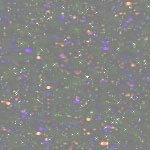
\includegraphics{fix.png}
\end{center}
\newpage
\item Random Noise

Random noise maybe the most common image noise. Random noise appear whenever were using high ISO
values.
Cameras has good at reducing the amount of random noise that is seen in photographs through technology.
The noise reduction feature on some cameras which remove random noise. So when technology continues to
improve, we can shoot in low light situation.

\begin{center}
	
\includegraphics{random.png}

\end{center}



\item Banding Noise

Banding noise is dependent on what type of camera we are using. With high end camera, we have never
seen banding noise. Some banding noise will appear when lower quality photograph are shot with higher
ISO value.
There are causes help banding noise appear: in the dark of photos or increase exposure too much and
digitally make a photograph too bright . We may also see more banding noise in certain white balances.

\begin{center}
	
\includegraphics{banding.png}
\end{center}

\end{itemize}

\subsection{Denoise}

Noise removal is very important task in image processing. It will help image restoration is to remove the
noise from the image in such a way that the original image is the best quality. In modern digital image
%processing, data denoising is a hard problem and it used to application areas. Noise removal is popular
solution for photography or improve the image was degraded.

\

Filtering is technique which can be decreasing or increasing an image. It’s the processed value for the
current pixel which depends on both itself and surrounding pixels. So filtering is a neighborhood operation,
it mean that the value of any given pixel in the output image is determined by applying some algorithm to the values of the pixels in the neighborhood of the corresponding input pixel. A pixel’s neighborhood is
some set of pixels, defined by their locations relative to that pixel.

\

Follow Image Processing, there are 4 type of filtering :

\begin{itemize}
\item Median Filter.

The median filter is a nonlinear digital filtering technique. So median filtering is very widely used in
image processing and it preserves edges while removing noise under certain conditions.
\item Average Filter.

The type of average filtering is simply to replace each pixel value in an image with the average value of its neighbors, including itself. This has the effect of eliminating pixel values which are unrepresentative
of their environment. Average filtering as a convolution filter.
\item Gaussian Filter.

In electronics and signal processing, filter whose impulse response is a Gaussian function (or an approximation
to it). Gaussian filters have feature of having no overshoot to a step function input while
minimizing the rise and fall time.
 
\item Wiener Filter

The main aim of this technique is to filter out noise that has corrupted the signal. It is kind of statistical
approach. For the designing of this filter one should know the spectral properties of the original signal
,the noise and linear time-variant filter whose output should be as close as to the original as possible.
The Wiener filter minimizes the mean square error between the estimated random process and the
desired process.
\end{itemize}


\vspace*{1cm}











\section{Report organization}

This part must explain how the report is organized.
